\chapter{File System}
\label{cap:FileSystem}
In questo capitolo facciamo una introduzione generale al concetto di
file system, mettendo in evidenza gli scopi e le varie
tipologie esistenti.
	\section{Introduzione concetto file System }
        	{\bf Definizione}: 
                \begin{quote}
		\textit{``Un file system è l'insieme dei tipi di dati
           astratti necessari per la memorizzazione, l'organizzazione
           gerarchica, la manipolazione, la navigazione, l'accesso e
           la lettura dei dati.''}
		\end{quote}
         Il file system è la componente del sistema operativo che si
         occupa dell'archiviazione dei dati sui dispositivi di
         memoria secondaria e terziaria, fornendo all'utente finale
         un interfaccia semplice da usare, realizzata mediante il
         concetto di \emph{File}.
         \newline \newline
               {\bf    Definizione}: 
	        \begin{quote}
                \textit{``I File è un insieme di informazioni, correlate e
           registrate in memoria secondaria, cui è stato assegnato un
           nome.''}
         \end{quote}
         Il file system si occupa dell'archiviazione dei file sulla
         memoria secondaria, gestisce le modalità di accesso a questi
         e si occupa anche della protezione dei file associando a essi
         dei privilegi.Tutto questo deve essere fatto in maniera
         trasparente rispetto all'utente finale che non deve avere
         nessuna conoscenza della posizione dei dati nel disco e ne
         come i dischi funzionino.
         \section{Struttura generale}
	 Per poter realizzare tutte queste funzionalità il file
         system è composto da molti livelli distinti. La struttura
         illustrata alla figura \ref{fig:Schema} è un esempio di struttura
         stratificata. Ogni livello si serve delle funzioni del
         livello inferiore per crearne di nuove per il livello
         superiore. 
		\begin{description}
		\item[File system base] Il File system di base è il livello più basso del file
		 system, questo modulo ha lo scopo di colloquiare con il
		 driver del disco inviando dei generici comandi di scrittura e
		 lettura. 
 		\end{description}
        
		\begin{description}
		\item[Il modulo di organizzazione dei file]
		Il  modulo di organizzazione dei file è a conoscenza
		dei file e dei loro blocchi logici, così come dei blocchi
		fisici dei dischi. Conoscendo il tipo di allocazione dei file
		usati e la locazione dei file, può tradurre gli indirizzi
		dei blocchi logici, che il file system di base deve trasferire
		negli indirizzi dei blocchi fisici.
		Il modulo di organizzazione dei file comprende anche il
		gestore dello spazio libero, che registra i blocchi non
		assegnati e li mette a disposizione del modulo di
		organizzazione dei file quando richiesto. 	
		\end{description}

		\begin{description}
		\item[File system logico]
		Il file system logico gestisce i metadati; si tratta
		di tutte le strutture del file system, eccetto gli effettivi
		dati (il contenuto dei file). Il file system logico gestisce
		le struttura  della directory per fornire al modulo di
		organizzazione dei file le informazioni di cui necessità,
		dato un nome simbolico di file. Mantiene le strutture dei
		file tramite i blocchi di controllo dei file (file control
		block,FCB), contenti informazioni sui file, come la
		proprietà,i permessi e la posizione del contenuto. 
                \end{description}
	 Nei file system stratificati la  duplicazione del codice è ridotta al minimo. Il controllo dell'IO e, talvolta, il codice di base del file system, possono 
	  essere comuni a numerosi file system, che poi gestiscono il file system logico e i moduli per l'organizzazione dei file secondo le proprie esigenze. 
          Sfortunatamente, la stratificazione può comportare un maggior overhead del sistema operativo, che può generare un conseguente decadimento delle prestazioni. 
         L'utilizzo della stratificazione e la scelta del numero di strati utilizzati sono aspetti critici nella realizzazione di un file system, in quanto queste scelte 
        incidono sulle prestazioni del sistema.         
	\begin{figure}[h]
 \centering
 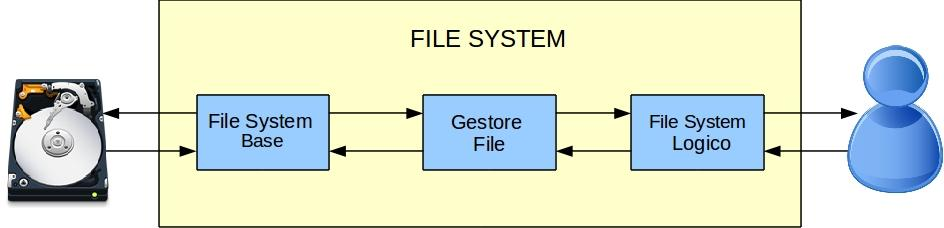
\includegraphics[width=350px,height=100px]{./Immagini/schema.jpg}
 % schema.jpg: 944x228 pixel, 96dpi, 24.98x6.03 cm, bb=0 0 708 171
 \caption{File system stratificato}
 \label{fig:Schema}
\end{figure}

	  \newpage
         \section{Strutture Dati}
         Per realizzare un file system si usano numerose strutture dati, sia nei dischi sia in memoria. Nei dischi, il file system tiene informazioni su come eseguire l'avviamento di un sistema operativo memorizzato nei dischi stessi, il numero totale di blocchi, il numero di locazioni dei blocchi liberi, la struttura delle directory e i singoli file. 
	 In questo paragrafo menzioniamo le più importanti : 
	  \begin{description}
	   \item[Blocco di controllo dell'avviamento] 
	    Il blocco di controllo di controllo dell'avviamento ({\emph boot control block}, contiene le informazioni necessarie al sistema per l'avviamento di un sistema operativo da quel volume; se il disco non contiene un sistema operativo, tale blocco è vuoto. Di solito è il primo blocco di un volume. 
 	  \end{description}
	  \begin{description}
	   \item[Blocchi di controllo dei volumi] 
	Il blocco di controllo dei volumi (\emph volume control block) ciascuno di loro contiene i dettagli riguardanti il relativo volume ( o partizione), come il numero e la dimensione dei blocchi nel disco, il contatore dei blocchi liberi e i relativi puntatori, il contatore dei blocchi di controllo dei file liberi e i relativi puntatori.
 	  \end{description}
	  \begin{description}
	   \item[Strutture delle directory]
	    La Struttura delle directory è la struttura che consente un organizzazione dei file secondo degli schemi logici, unica per ogni volume. 
 	  \end{description}
	  \begin{description}
	   \item[Blocchi di controllo di file]
	    I blocchi di controllo di file {\emph (FCB)}, contiene molti dettagli dei file, compresi i permessi di accesso ai relativi file, i proprietari, le dimensioni e la locazione dei blocchi di dati. 
 	  \end{description}
	  Le informazioni tenute in memoria servono sia per la gestione del file sytem sia per migliorare le prestazioni attraverso l'uso di cache. Questi dati vengono caricati in memoria 
	quando il volume è montato ed eliminati nel momento nel quale viene smontato. 
	    \begin{description}
	     \item[Tabella di montaggio]
	      La tabella di montaggio interna alla memoria che contiene tutte le informazioni attinenti al ciascun volume montato. 
 	    \end{description}
	    \begin{description}
	     \item[Struttura delle Directory]
	      Una parte della struttura delle directory presente nel disco viene carica in memoria in base a quali directory i processi hanno avuto accesso di recente.
 	    \end{description}
	    \begin{description}
	     \item[Tabella generale file aperti]
	      La tabella generale dei file aperti  contiene una coppia del FCB per ciascun file aperto all'interno del sistema operativo.  
 	    \end{description}
	      \begin{description}
	       \item[Tabella locale file aperti] 
		La tabella locale dei file aperti è una struttura dati associata ad ogni processo che contiene tutte le informazioni attinenti hai file aperti da quel determinato processo, tipicamente mantiene dei puntatori ai FCB della tabella globale dei file aperti. 
 	      \end{description}
         \section{Metodi di allocazione} 
         Il problema principale che il file system deve risolvere è l'allocazione dello spazio per i file nel disco. Questo è un problema complesso da cui dipende l'efficienza del file system stesso, perché un file system efficiente deve fornire una gestione dello spazio ottimale riducendo al minimo gli overhead e un accesso rapido al contenuto dei file. 
         Esistono tre metodi principali per l'allocazione dei file, ognuno con i suoi vantaggi e svantaggi,in base alle esigenze che si hanno e il contesto nel quale il file system andrà a lavorare si adotterà il metodo più idoneo.
         
      \begin{description}
       \item[Allocazione contigua]
        La base di questo metodo di allocazione consiste nell'occupare per ogni file un insieme di blocchi contigui del disco. Il principale vantaggio di questo metodo di allocazione è che si rendono trascurabili il numero di posizionamenti  richiesti per accedere al contenuto del file , così come è trascurabile il tempo di ricerca quando quest'ultimo è necessario.
      Il primo problema di cui è affetto questo metodo è l'individuazione dello spazio libero, in quanto il gestore dello spazio libero deve trovare uno spazio libero formato da blocchi contigui che sia in grado di contenere la quantità di dati da immagazzinare, per fare questo si possono usare degli algoritmi per la scelta del buco libero ( esempi sono best-fit las-fit first-fit), ma tutti questi sono affetti dal problema della frammentazione esterna. 
      Il secondo problema che si presenta usando questo metodo è che può risultare impossibile estendere il file dopo il suo allocamento, in quanto lo spazio oltre le due estremità del file può essere già in uso, quindi non è possibile ampliare il file in modo continuo.
      Questa metodologia può essere affiancata da varie estensioni per renderla in grado di affrontare i problemi precedenti. 
      Questo modello di allocazione è molto efficiente come tempi di accesso ai dati, ma le problematiche attinenti alla frammentazione dello spazio lo rendono usabile solo in particolari condizioni, e anche con l'introduzione di varie estensioni questi problemi vengono ridotti ma non eliminati. 
       \end{description}

      \begin{description}
       \item[Allocazione Concatenata]
        Il metodo di allocazione Concatenata risolve tutti i problemi di cui era afflitto il metodo di allocazione contigua.Con questo tipo di allocazione, infatti , ogni file è composto da una lista concatenata di blocchi del disco i quali possono essere sparsi in qualsiasi punto del disco stesso. Per poter risalire a un file nel disco la directory deve contenere 
        un puntatore al primo blocco, e ogni blocco contiene il puntatore al blocco successivo fino all'ultimo blocco della lista, che conterrà un puntatore  speciale che indicherà che questo è l'ultimo blocco. Quindi per eseguire la lettura si legge l'indirizzo del primo blocco  dalla directory fino a raggiungere la posizione ricercata mediante la lista di blocchi.
        Il primo problema di questo metodo è che i file possono essere usati in modo efficiente solo con accessi sequenziali, mentre l'accesso diretto al file estremamente inefficiente in quanto bisogna scorrere tutta la lista di blocchi prima di arrivare alla posizione ricercata. 
        Un altro svantaggio è lo spazio richiesto per il salvataggio dei puntatori dei vari blocchi. La soluzione più comune a questo problema consiste nel riunire un certo numero di blocchi contigui in {\bf cluster}, e nell'allocare cluster invece di blocchi. Questa soluzione però incrementa la frammentazione interna che era minore con l'allocazione di blocchi.
        Il secondo problema riguarda l'affidabilità. Essendo i file gestiti mediante liste se si corrompe un puntatore si ha la perdita del file in quanto non è più possibile seguire la lista. Esistono varie soluzioni a questo problema, la prima consiste nell'usare liste doppiamente concatenate, oppure usare una gestione ridondante dei puntatori. 
        Un'importante versione del metodo di allocazione Concatenata e quello {\bf FAT} che verrà analizzato in dettaglio nel paragrafo §\ref{cap:Fat}, questo risolve in modo efficiente il problema dell'accesso in modo diretto. 
       \end{description}
      \begin{description}
        \item[Allocazione indicizzata]
        Il metodo di allocazione indicizzata risolve il problema, raggruppando i puntatori in una sola locazione che prende il nome di {\bf blocco indice}. Ogni file ha il proprio blocco indice, si tratta di un array  d'indirizzi di blocchi del disco. L'\textit{i}-esimo elemento del blocco indice punta all'\textit{i}-esimo blocco del file. Per poter risalire al file,la directory contiene il puntatore al blocco indice del file. Con questa soluzione sono efficienti sia gli accessi sequenziali,  che gli accessi diretti e in più non si ha frammentazione esterna.
        Anche questo metodo di allocazione è afflitto da una problematica, che consiste nello scegliere la grandezza del blocco indice, infatti se si sceglie una grandezza troppo piccola non si possono allocare file di grandi dimensioni, invece se si sceglie una grandezza del blocco indice troppo elevata si introduce uno spreco di spazio perché la maggior parte dei puntatori interni del blocco indice rimangono inutilizzati. 
        Per gestire questa situazione si usano vari approcci : 
        \begin{itemize}
         \item \textbf{Schema concatenato} Un blocco indice è formato da un solo blocco del disco, e per realizzare più blocchi vengono concatenati più blocchi indice tra loro.
        \end{itemize}
        \begin{itemize}
         \item \textbf{Indice a più livelli} Un blocco indice di primo livello punta ai blocchi indice di secondo livello che, a loro volta, puntano ai blocchi dei file, così si crea una struttura ad albero che permette l'allocazione di grandi file.
        \end{itemize}
        \begin{itemize}
         \item \textbf{Schema combinato} Consiste nell'utilizzare entrambe le soluzioni precedenti, associando ad ogni file dei puntatori diretti ai blocchi dei file , e dei puntatori a blocchi indice di vario livello in base alle esigenze. In questo modo con gli indirizzamenti diretti si possono gestire i file di piccole dimensioni senza introdurre rilevanti perdite di spazio, e quando lo spazio indirizzato da questi risulta insufficiente, si utilizzano i blocchi indice a più livelli. 
        \end{itemize}
        \end{description}
         Come esposto esistono una varietà di metodi di allocazione dei dati sul disco, ognuno di questi ha i suoi vantaggi e svantaggi. Il metodo di allocazione da adottare in un file system  è legato al  contesto in cui andrà a lavorare quel file system, soprattutto con quale tipologia di file, così facendo  si cerca di ottimizzare al meglio le prestazioni.
         Spesso però questo non è sufficiente, e per ottenere dei file system efficienti, bisogna inserire delle estensioni per migliorarne le prestazioni, alle volte a discapito della generalità del file system steso.
         \section{Metodi di gestione dello spazio libero} 
         Un altro aspetto importante del file system  è la gestione dello spazio libero. Il sistema deve conservare una lista dello spazio libero dove sono registrate tutte le locazioni libere del disco. Per creare un file occorre cercare nella lista dello spazio libero la quantità di spazio necessaria e assegnarla al nuovo file, quindi rimuovere questo spazio dalla lista. Quando si cancella un file, si aggiungono alla lista dello spazio libero i blocchi del disco ad esso assegnati. 
         La lista dello spazio libero può essere implementata in vari modi: 
         \begin{itemize}
          \item \textbf{Mappa di BIT} Con questo metodo si realizza la lista mediante \textit{una mappa di bit}.Ogni blocco è rappresentato da un bit: se il blocco è libero, il bit è 1, se il bit è assegnato il bit è 0. Il vantaggio principale è che il metodo è molto semplice da realizzare ed efficiente.
         \end{itemize}
          \begin{itemize}
           \item \textbf{Lista concatenata} Con questo metodo si collegano tutti i blocchi liberi, e si tiene un puntatore al primo blocco libero in una particolare posizione del disco. Quando si ha necessità di un blocco si preleva  semplicemente il primo della lista.Questo metodo non è efficiente se si ha necessità di scorrere la lista dei blocchi.    
          \end{itemize}
          \begin{itemize}
           \item\textbf{ Conteggio} Questo metodo, sfrutta l'idea che più blocchi liberi siano contigui tra di loro, in questo modo si può tenere traccia dell'indirizzo del primo blocco ed il numero di blocchi liberi contigui che seguono il primo blocco, e anche se la coppia indirizzo più contatore occupano più di un indirizzo normale, la lista finale comunque ha una lunghezza inferiore.
          \end{itemize}
            Come nel caso  della scelta del metodo di allocazione anche qui bisogna scegliere l'implementazione in base al contesto in cui ci andrà a lavorare.
         \section{Conclusioni}
            Come si è visto in questa sezione il file system è un oggetto complesso di fondamentale importanza per il sistema operativo.  Il processo di realizzazione di un file system è molto lungo è complesso, e deve essere curato nei minimi particolari per cercare di ridurre al minimo gli errori, si pensi alle conseguenze che avrebbero degli errori di programmazione su una parte così delicata del sistema, si potrebbero avere  perdite di dati, accessi non autorizzati ai file e così via.
            Nella scelta del file system da implementare abbiamo scelto il FAT per la sua semplicità implementativa tralasciando le prestazioni in quanto il contesto in cui lavorerà è un semplice sistema didattico. 

\clearpage{\pagestyle{empty}\cleardoublepage}

%%% Local Variables: 
%%% mode: latex
%%% TeX-master: "tesi"
%%% End: 
